\justifying \small 

\textcolor{orange}{\#include <stdio.h>} 
\textcolor{orange}{\#include "octal\_hex\_2.c"} 
\textcolor{gray}{/**
 * Probando numeros reales, octales
 * y hexadecimales
 * @return
 */} 
\textcolor{cyan}{int} 
\textcolor{white}{main} 
\textcolor{magenta}{(} 
\textcolor{magenta}{)} 
\textcolor{magenta}{\{} 
\textcolor{gray}{// Declaracion de un numero real} 
\textcolor{cyan}{float} 
\textcolor{white}{\_n} 
\textcolor{yellow}{=} 
\textcolor{green}{-.5e+12} 
\textcolor{magenta}{;} 
\textcolor{white}{printf} 
\textcolor{magenta}{(} 
\textcolor{green}{"\%f \textbackslash n"} 
\textcolor{magenta}{,} 
\textcolor{white}{\_n} 
\textcolor{magenta}{)} 
\textcolor{magenta}{;} 
\textcolor{white}{\_n} 
\textcolor{yellow}{*=} 
\textcolor{green}{2.e-1} 
\textcolor{magenta}{;} 
\textcolor{gray}{/* multiplicado por  */} 
\textcolor{white}{printf} 
\textcolor{magenta}{(} 
\textcolor{green}{"\%f \textbackslash n"} 
\textcolor{magenta}{,} 
\textcolor{white}{\_n} 
\textcolor{magenta}{)} 
\textcolor{magenta}{;} 
\textcolor{cyan}{int} 
\textcolor{white}{hexadecimal} 
\textcolor{yellow}{=} 
\textcolor{green}{0x31f} 
\textcolor{magenta}{;} 
\textcolor{gray}{/* representa 799 en decimal */} 
\textcolor{cyan}{int} 
\textcolor{white}{hexadecimal\_2} 
\textcolor{yellow}{=} 
\textcolor{green}{0X1a2} 
\textcolor{magenta}{;} 
\textcolor{gray}{/* representa 418 en decimal */} 
\textcolor{white}{printf} 
\textcolor{magenta}{(} 
\textcolor{green}{"hexadecimal 1: \%d\textbackslash n"} 
\textcolor{magenta}{,} 
\textcolor{white}{hexadecimal} 
\textcolor{magenta}{)} 
\textcolor{magenta}{;} 
\textcolor{white}{printf} 
\textcolor{magenta}{(} 
\textcolor{green}{"hexadecimal 2: \%d\textbackslash n"} 
\textcolor{magenta}{,} 
\textcolor{white}{hexadecimal\_2} 
\textcolor{magenta}{)} 
\textcolor{magenta}{;} 
\textcolor{white}{hexadecimal\_2} 
\textcolor{yellow}{++} 
\textcolor{magenta}{;} 
\textcolor{white}{hexadecimal} 
\textcolor{yellow}{+=} 
\textcolor{white}{hexadecimal\_2} 
\textcolor{magenta}{;} 
\textcolor{white}{printf} 
\textcolor{magenta}{(} 
\textcolor{green}{"resultado: \%d\textbackslash n"} 
\textcolor{magenta}{,} 
\textcolor{white}{hexadecimal} 
\textcolor{magenta}{)} 
\textcolor{magenta}{;} 
\textcolor{gray}{// Salida 916} 
\textcolor{cyan}{int} 
\textcolor{white}{octal\_1} 
\textcolor{yellow}{=} 
\textcolor{green}{023} 
\textcolor{magenta}{;} 
\textcolor{gray}{/* representa 19 
    en decimal */} 
\textcolor{cyan}{int} 
\textcolor{white}{octal\_2} 
\textcolor{yellow}{=} 
\textcolor{green}{0176} 
\textcolor{magenta}{;} 
\textcolor{gray}{/* representa 126
    en decimal */} 
\textcolor{white}{printf} 
\textcolor{magenta}{(} 
\textcolor{green}{"octal 1: \%d\textbackslash n"} 
\textcolor{magenta}{,} 
\textcolor{white}{octal\_1} 
\textcolor{magenta}{)} 
\textcolor{magenta}{;} 
\textcolor{white}{printf} 
\textcolor{magenta}{(} 
\textcolor{green}{"octal 2: \%d\textbackslash n"} 
\textcolor{magenta}{,} 
\textcolor{white}{octal\_2} 
\textcolor{magenta}{)} 
\textcolor{magenta}{;} 
\textcolor{white}{printf} 
\textcolor{magenta}{(} 
\textcolor{green}{"resultado: \%d\textbackslash n"} 
\textcolor{magenta}{,} 
\textcolor{magenta}{(} 
\textcolor{white}{octal\_1} 
\textcolor{yellow}{+} 
\textcolor{white}{octal\_2} 
\textcolor{magenta}{)} 
\textcolor{magenta}{)} 
\textcolor{magenta}{;} 
\textcolor{white}{multiplicar} 
\textcolor{magenta}{(} 
\textcolor{magenta}{)} 
\textcolor{magenta}{;} 
\textcolor{white}{piramide} 
\textcolor{magenta}{(} 
\textcolor{green}{10} 
\textcolor{magenta}{)} 
\textcolor{magenta}{;} 
\textcolor{cyan}{return} 
\textcolor{green}{0} 
\textcolor{magenta}{;} 
\textcolor{magenta}{\}} 




\begin{frame}{Histograma Tokens Usados} 
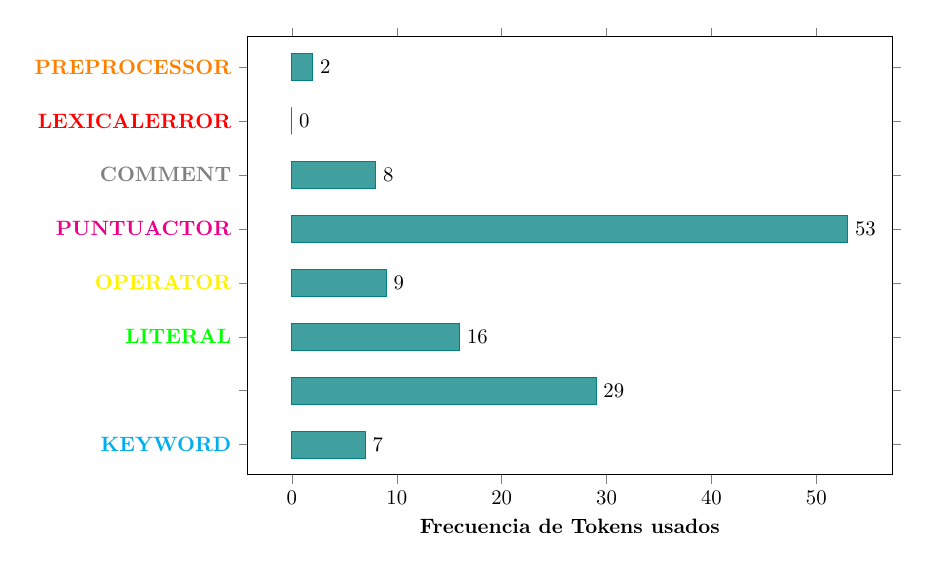
\begin{tikzpicture}[scale=0.75] % tamaño 
\begin{axis}[xbar,tick align=outside, 
    width=12.5cm,       % largo 
    height=9cm,       % altura 
    bar width={13pt},   % grosor linea 
    enlargelimits=0.08, % cercania a linea 
    nodes near coords, 
    nodes near coords align=horizontal, 
    point meta=x * 1, % The displayed number. 
    xlabel=\textbf{Frecuencia de Tokens usados}, 
    ytick={0,...,7}, 
    yticklabels={ 
        \textcolor{cyan}{\textbf{KEYWORD}},         % POSITION 0 
        \textcolor{white}{\textbf{IDENTIFIER}},     % POSITION 1 
        \textcolor{green}{\textbf{LITERAL}},        % POSITION 2 
        \textcolor{yellow}{\textbf{OPERATOR}},      % POSITION 3 
        \textcolor{magenta}{\textbf{PUNTUACTOR}},   % POSITION 4 
        \textcolor{gray}{\textbf{COMMENT}},         % POSITION 5 
        \textcolor{red}{\textbf{LEXICALERROR}},     % POSITION 6 
        \textcolor{orange}{\textbf{PREPROCESSOR}}   % POSITION 7 
    }] 
\addplot 
[draw=teal,fill=teal!75] 
coordinates {(7,0) (29,1) (16,2) (9,3) (53,4) (8,5) (0,6) (2,7)}; 
\end{axis}
\end{tikzpicture}
\end{frame}
